\chapter{Background and Literature Review}

\section{Workflow Automation}

Workflow automation, in the context of web applications, is the practice of orchestrating sequences of operations across multiple independent services in response to real-world events, without requiring a human to initiate each operation. A workflow typically consists of a \emph{trigger}, which is the event that starts the workflow, and one or more \emph{actions}, which are the operations performed in response. A collection of such rules is usually referred to as a \emph{Zap}, a \emph{recipe}, or a \emph{scenario}, depending on the commercial platform.

\subsection{Webhooks}

A webhook is an HTTP callback: an endpoint hosted by an application that another application can POST to in order to notify the first application that an event has occurred. Because webhooks are implemented using ordinary HTTP, they are universally supported across programming languages and cloud services, and require no special client libraries. In the platform presented in this report, the only supported trigger type is a webhook: the platform publishes a unique URL for each workflow, and any external service that wishes to fire the workflow simply performs an HTTP POST to that URL with an arbitrary JSON body. This body, called the webhook payload, becomes available as input data to each of the workflow's actions.

\subsection{Triggers and Actions}

In the data model of a workflow automation platform, a \emph{trigger} is the data structure that specifies what should start a workflow, while an \emph{action} specifies what should happen as a result. Every action has an associated \emph{action type}, which describes the kind of operation (e.g.\ send an email, forward an HTTP request, insert a row into a spreadsheet) and the metadata schema required to parameterise it. Each action instance stores the concrete parameters supplied by the user: for instance, the recipient address of the email, or the destination wallet for a blockchain transfer. Multiple actions may be attached to a single workflow and are executed in a user-specified order.

\section{Microservices Architecture}

The microservices architectural style, popularised by Fowler and Lewis~\cite{fowler2014microservices} and subsequently applied at large scale by companies such as Netflix and Amazon, decomposes a single application into a set of small services, each responsible for a well-defined business capability. Services communicate over the network, typically using HTTP for synchronous calls or an event broker for asynchronous messaging. Each service can be developed, deployed and scaled independently of the others.

For a workflow automation platform, a microservices architecture offers several concrete advantages:

\begin{itemize}
\item The component responsible for receiving webhooks must remain highly available and respond quickly; separating it from the component that executes actions (which may take seconds or minutes) allows each to be scaled and tuned independently.
\item The execution of an action may fail for reasons unrelated to the rest of the system (an external API being down, a rate limit, a transient network error). Isolating action execution in a separate worker service prevents such failures from affecting the API surface presented to the user.
\item Different components benefit from different deployment strategies: stateless API services can be replicated behind a load balancer, while stateful consumers can be horizontally scaled across Kafka partitions.
\end{itemize}

\section{Transactional Outbox Pattern}

A recurring problem when integrating a relational database with a message broker is ensuring that a business state change and the corresponding outgoing message are both persisted, or neither are. A naive implementation, in which the service first writes to the database and then publishes to the broker, suffers from \emph{dual-write} inconsistency: a crash or network failure between the two writes leaves the system in a state where the database has been updated but no message was produced, or the opposite. Over time these inconsistencies accumulate and undermine the reliability of the platform.

The \emph{transactional outbox} pattern, documented as part of the broader catalogue of microservices patterns by Richardson~\cite{richardson2018microservices} and elaborated online at the \texttt{microservices.io} pattern repository~\cite{microservicesio_outbox}, solves this problem by persisting the outgoing message as part of the same database transaction that records the business state change. The message is written into a dedicated \emph{outbox} table rather than being sent directly to the broker. A separate process, sometimes called the \emph{message relay} or \emph{outbox poller}, asynchronously reads new rows from this table, publishes their contents to the broker, and then deletes (or marks as processed) the row. Because both writes occur inside a single database transaction, atomicity is guaranteed by the relational database itself and no distributed transaction coordinator is required. A conceptual view of the pattern is shown in Figure~\ref{fig:outbox-pattern}.

\begin{figure}[h]
\centering
\begin{tikzpicture}[
    node distance=1.2cm,
    box/.style={draw, thick, minimum width=2.2cm, minimum height=0.95cm, align=center, rounded corners=2pt, font=\small},
    db/.style={draw, thick, cylinder, shape border rotate=90, aspect=0.25, minimum width=2.2cm, minimum height=1.4cm, align=center, font=\small},
    >={Stealth[length=2mm]}
]
\node[box] (app) {Application\\Service};
\node[db, right=1.3cm of app] (database) {Database\\(business\\+ outbox)};
\node[box, right=1.3cm of database] (relay) {Message\\Relay};
\node[box, right=1.3cm of relay] (broker) {Message\\Broker};

\draw[->, thick] (app)      -- node[above, font=\scriptsize] {single txn}  (database);
\draw[->, thick] (database) -- node[above, font=\scriptsize] {poll outbox} (relay);
\draw[->, thick] (relay)    -- node[above, font=\scriptsize] {publish}     (broker);
\end{tikzpicture}
\caption{Conceptual overview of the transactional outbox pattern.}
\label{fig:outbox-pattern}
\end{figure}

The platform developed in this project adopts the transactional outbox pattern in its webhook ingestion path. Each incoming webhook produces one \texttt{ZapRun} row and one \texttt{ZapRunOutbox} row, both inserted inside a single database transaction. A dedicated processor service, described in Chapter~4, is responsible for polling the outbox table and relaying its contents to Apache Kafka. The pattern provides the platform with \emph{at-least-once} delivery semantics for every webhook received, irrespective of transient failures in either the processor or the broker.

\section{Apache Kafka and Event Streaming}

Apache Kafka~\cite{kafka_docs} is a distributed, partitioned, replicated log that serves as the messaging backbone of the platform. Producers write records to named \emph{topics}, which are subdivided into \emph{partitions}; consumers belonging to a \emph{consumer group} read records from those partitions, with Kafka guaranteeing that each partition is consumed by at most one member of the group at any given time. Consumer offsets are stored inside Kafka itself, allowing a consumer to resume exactly where it left off after a restart.

Kafka was chosen over alternatives such as RabbitMQ or Redis Streams for three reasons that are directly relevant to this project. First, Kafka persists all records on disk for a configurable retention period, so messages survive consumer crashes and can be replayed during development and debugging. Second, Kafka's partitioning model provides a natural unit of horizontal scalability: adding more worker instances to the consumer group immediately distributes the load. Third, Kafka's wide industrial adoption means that the platform's operational patterns, such as consumer-group rebalancing, dead-letter queues and log compaction, map cleanly onto concepts already familiar to practitioners.

Figure~\ref{fig:kafka-pubsub} illustrates the basic publish-subscribe abstraction provided by Kafka. A \emph{producer} writes records into a named \emph{topic} (here, a topic called \emph{payment}), where each record is appended to the end of the log and assigned a monotonically increasing \emph{offset}. One or more \emph{consumers} read records from the topic at their own pace and track their progress using these offsets, which means that adding a new consumer never disturbs the existing ones. In the diagram, two independent consumers, ``Send SMS'' and ``Send Email'', each receive every record published to the topic.

\begin{figure}[h]
\centering
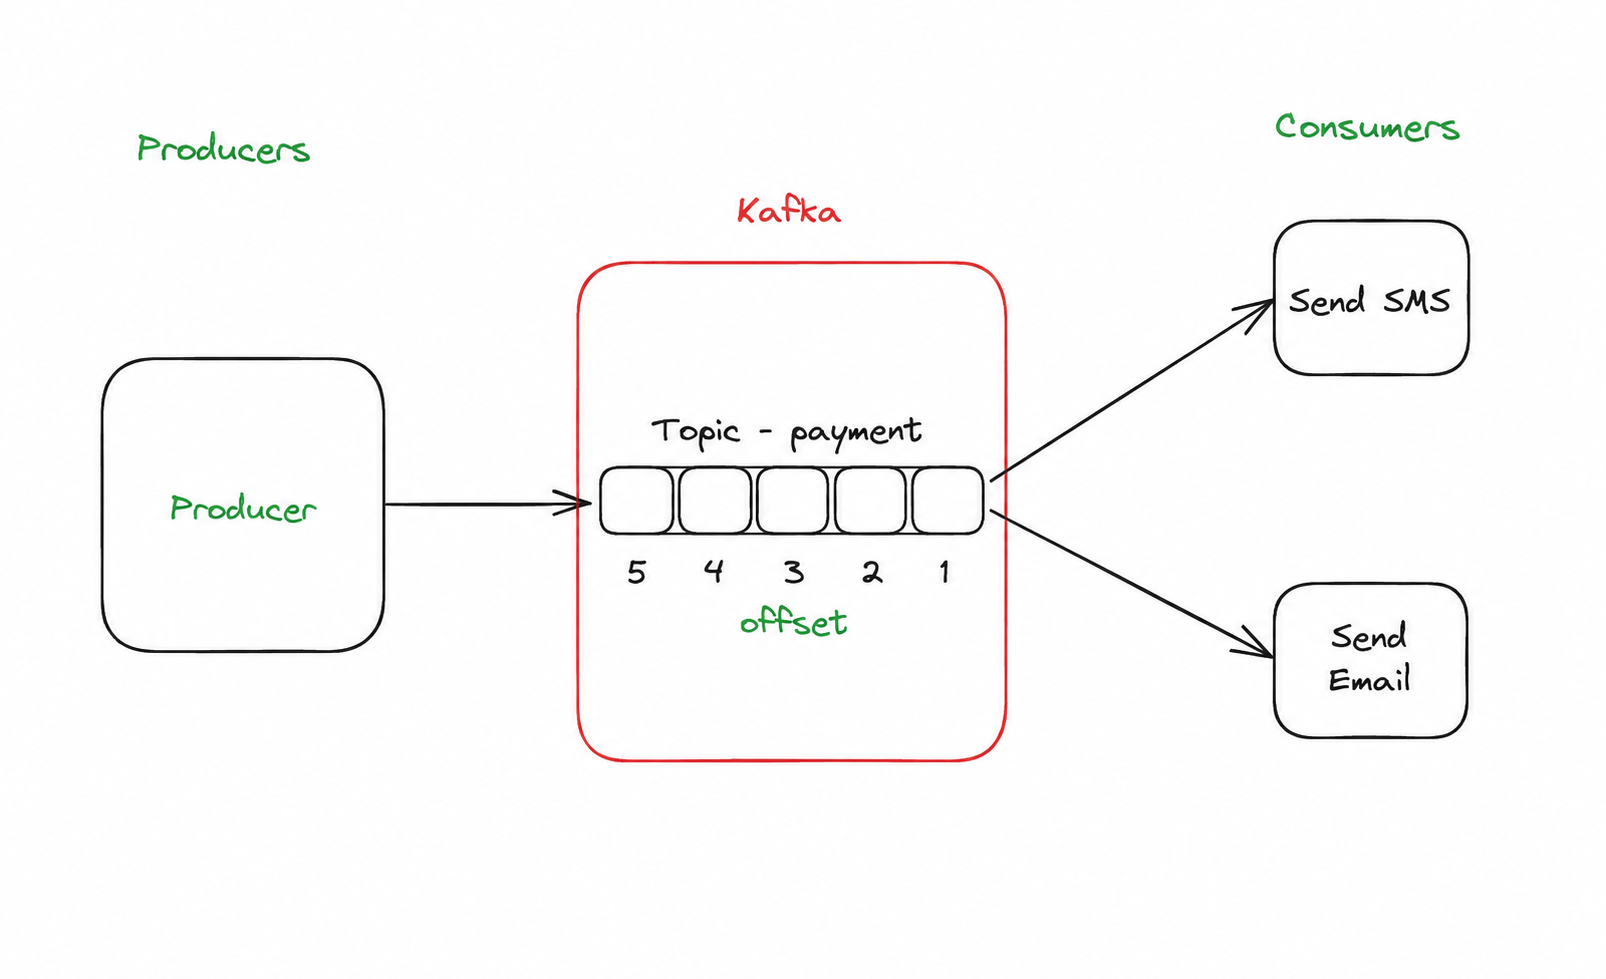
\includegraphics[width=0.85\textwidth]{figures/kafka-pub-sub.png}
\caption{Publish-subscribe model in Apache Kafka, with one producer, a single-partition topic and two independent consumers.}
\label{fig:kafka-pubsub}
\end{figure}

A practical example of how this abstraction enables decoupled, event-driven design is shown in Figure~\ref{fig:event-driven-flow}. A user-facing payment is recorded by a Node.js backend, which then writes a single event to Kafka. Three downstream services -- an email service, a mobile-SMS service and a push-notification service -- each independently consume that event and perform their respective side effects. The producer has no awareness of how many consumers exist or what they do, and additional consumers can be introduced later without modifying the producer. The platform developed in this project applies the same pattern: the processor service is the producer, and the worker service (which can be horizontally scaled) is the consumer of action events.

\begin{figure}[h]
\centering
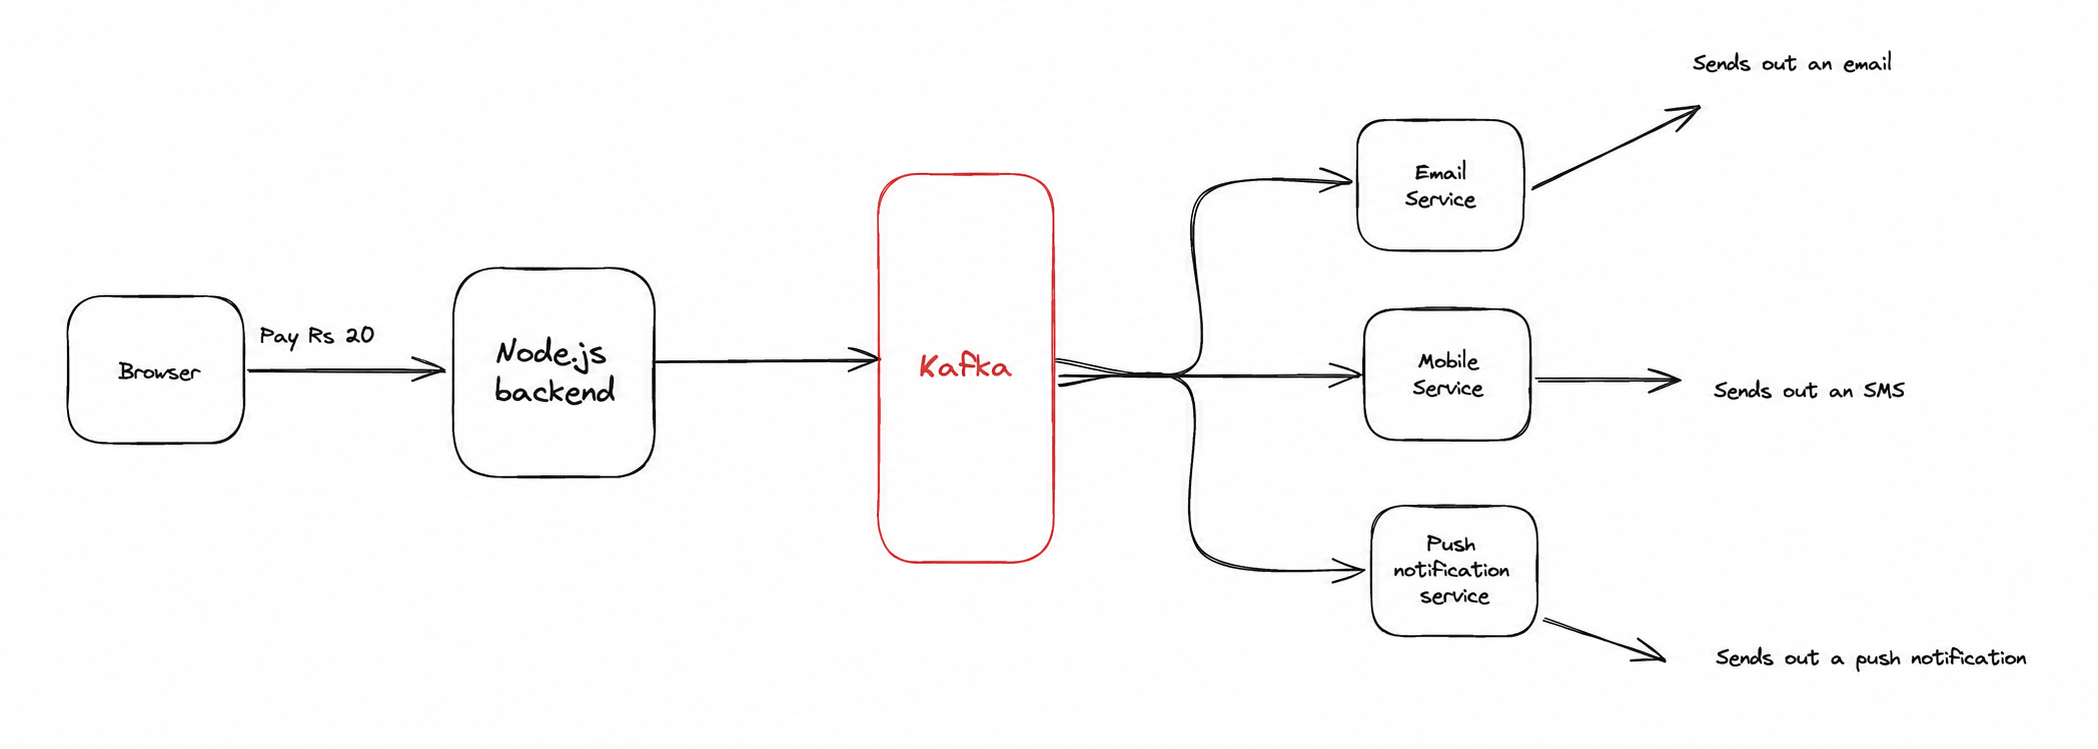
\includegraphics[width=\textwidth]{figures/event-driven-flow.png}
\caption{Event-driven fan-out via Kafka: a single payment event is consumed independently by an email service, a mobile service and a push-notification service.}
\label{fig:event-driven-flow}
\end{figure}

\section{Supporting Technologies}

The platform is built on top of several additional open-source technologies. The frontend is implemented using Next.js~\cite{nextjs_docs}, a React-based framework that supports both server-side rendering and static generation and provides built-in routing and API endpoints. The backend services are implemented in TypeScript on top of Node.js and the Express framework, with input validation performed using Zod schemas. Database access is mediated through Prisma ORM~\cite{prisma_docs}, which provides a fully typed query builder and an automatic migration system. Authentication is based on JSON Web Tokens~\cite{jones2015jwt}, with passwords hashed using the bcrypt algorithm. Transactional emails are sent using Nodemailer over standard SMTP, while blockchain actions interact with the Solana network through the \texttt{@solana/web3.js} library. The entire system is containerised using Docker and orchestrated locally with Docker Compose.
